\section{Cadenas de Markov}

\subsection{}

\begin{frame}%\frametitle{Ejemplos de matrices}
	
	\begin{ejer}{\textbf{Cadena de Markov}}\justifying 
		Un equipo de investigación de mercado realiza un estudio controlado para determinar
		cuáles marcas de celular prefieren las personas. La muestra consiste de 200 personas, y a cada una
		se le pide probar dos marcas (Samsung y iPhone) durante un periodo de varios meses. Con base
		en las respuestas de la encuesta, el equipo de investigación compila las siguientes estadísticas 
		acerca de las preferencias de celulares.
		\begin{enumerate}
			\item[\labelname{$a$}] De quienes usan Samsung en cualquier mes, 70\% siguen usándolo el mes siguiente,
			mientras que el 30\% cambia a iPhone.
			\item[\labelname{$a$}] De quienes usan iPhone en cualquier mes, 80\% siguen usándolo el mes siguiente, 
			mientras que el 20\% cambian a Samsung.
		\end{enumerate}
		Suponga que cuando inicia el estudio 120 personas usan Samsung y 80 personas usan iPhone. 
		¿Cuántas personas usarán cada marca 1 mes después? ¿Y 2 meses después? ¿Y un año después?
	\end{ejer}
	
	\vspace{-5mm}
	
	\begin{columns}[c]
		\hspace{-0.5cm}
		\begin{column}{0.6\textwidth}
			% http://texample.net/tikz/examples/graph/
			\GraphInit[vstyle = Shade]
			\tikzset{
				LabelStyle/.style = { rectangle, rounded corners, draw,
					minimum width = 1em, fill = yellow!20,
					text = red, font = \bfseries },
				VertexStyle/.append style = { inner sep=2pt,
					font = \Large\bfseries},
				EdgeStyle/.append style = {->, bend left} }
			\begin{center}
				\begin{tikzpicture}[thick,scale=0.4, every node/.style={scale=0.8}]
				\SetGraphUnit{6}%\pause 
				\Vertex{i}
				\WE(i){S}
				\EA(S){i}%\pause \pause 
				\Loop[dist = 5cm, dir = NO, label = 70\%](S.west)%\pause
				\tikzset{EdgeStyle/.append style = {bend left = 60}}%\pause 
				%\Edge[label = 30\%](S)(i)%\pause\pause  
				% Workaround: https://tex.stackexchange.com/a/397326
				\begin{scope}[/tikz/handle active characters in nodes=false]
					\Edge[label = 30\%](S)(i)%\pause\pause  
				\end{scope}
				\Loop[dist = 5cm, dir = SO, label = 80\%](i.east)%\pause\pause 
				\begin{scope}[/tikz/handle active characters in nodes=false]
					\Edge[label = 20\%](i)(S)
				\end{scope}
				\end{tikzpicture}
			\end{center}					
		\end{column}
		\hspace{-1.2cm}
		\begin{column}{0.4\textwidth}
			\[	
				\begin{array}{c@{}}
					\rowind{\color{blue}Siguiente} 
				\end{array}
				\begin{array}{c@{}c@{}}
					\rowind{\textbf{S}} \\ \rowind{\textbf{i}} 
				\end{array}
				\mathop{\left(
						\begin{array}{ *{2}{c} }
						\colind{0.7}{\textbf{S}}  &  \colind{0.2}{\textbf{i}} \\[0mm]			
						0.3 & 0.8    
						\end{array}
						\right)}^{
						\begin{array}{@{}c@{}}
						\rowind{\color{blue}Presente} \\ \mathstrut
						\end{array}
						}
			\]
		\end{column}	
	\end{columns}
		
\end{frame}

%%------------------------------------------------------------------------------------------------------

\subsection{}

{\nologo
\begin{frame}\frametitle{Al incio 120 usan Samsung y 80 usan iPhone}
		
		\vspace{-6mm}
		
		\begin{columns}[c]
		\hspace{-0.5cm}
		\begin{column}{0.6\textwidth}
			% http://texample.net/tikz/examples/graph/
			\GraphInit[vstyle = Shade]
			\tikzset{
				LabelStyle/.style = { rectangle, rounded corners, draw,
					minimum width = 1em, fill = yellow!20,
					text = red, font = \bfseries },
				VertexStyle/.append style = { inner sep=2pt,
					font = \Large\bfseries},
				EdgeStyle/.append style = {->, bend left} }
			\begin{center}
				\begin{tikzpicture}[thick,scale=0.4, every node/.style={scale=0.8}]
				\SetGraphUnit{6}%\pause 
				\Vertex{i}
				\WE(i){S}
				\EA(S){i}%\pause \pause 
				\Loop[dist = 5cm, dir = NO, label = 70\%](S.west)%\pause
				\tikzset{EdgeStyle/.append style = {bend left = 60}}%\pause 
				% Workaround: https://tex.stackexchange.com/a/397326
				\begin{scope}[/tikz/handle active characters in nodes=false]
					\Edge[label = 30\%](S)(i)%\pause\pause  
				\end{scope}	
				\Loop[dist = 5cm, dir = SO, label = 80\%](i.east)%\pause\pause 
				\begin{scope}[/tikz/handle active characters in nodes=false]
					\Edge[label = 20\%](i)(S)
				\end{scope}	
				\end{tikzpicture}
			\end{center}					
		\end{column}
		\hspace{-1.2cm}
		\begin{column}{0.4\textwidth}
			\[	
			\begin{array}{c@{}}
			\rowind{\color{blue}Siguiente} 
			\end{array}
			\begin{array}{c@{}c@{}}
			\rowind{\textbf{S}} \\ \rowind{\textbf{i}} 
			\end{array}
			\mathop{\left(
				\begin{array}{ *{2}{c} }
				\colind{0.7}{\textbf{S}}  &  \colind{0.2}{\textbf{i}} \\[0mm]			
				0.3 & 0.8    
				\end{array}
				\right)}^{
				\begin{array}{@{}c@{}}
				\rowind{\color{blue}Presente} \\ \mathstrut
				\end{array}
			}
			\]
		\end{column}	
	\end{columns}	
	
	\vspace{-0mm}
	\begin{itemize}
		
		\item Número de usuarios de Samsung y de iphone resp., despues de 1 mes:
		
		\vspace{-3mm}
		\[	
		\begin{array}{c@{\hspace{0.7\tabcolsep}}c@{\hspace{0.7\tabcolsep}}c@{\hspace{0.7\tabcolsep}}c@{\hspace{0.7\tabcolsep}}c}
		0.70({\color{ForestGreen}120}) & + & 0.20({\color{ForestGreen}80}) & = & 100 \\[1mm]
		0.30({\color{ForestGreen}120}) & + & 0.80({\color{ForestGreen}80}) & = & 100 \\
		\end{array}
		\quad \Leftrightarrow \quad 
		\left(
		\begin{array}{@{\hspace{0.2\tabcolsep}}c@{\hspace{1.2\tabcolsep}}c@{\hspace{0.2\tabcolsep}}}
		0.70 & 0.20 \\[1mm]
		0.30 & 0.80
		\end{array}
		\right)
		\left(
		\begin{array}{@{\hspace{0.2\tabcolsep}}c@{\hspace{0.2\tabcolsep}}}
		{\color{ForestGreen}120} \\[1mm]
		{\color{ForestGreen}80}
		\end{array}
		\right)
		=
		\left(
		\begin{array}{@{\hspace{0.2\tabcolsep}}c@{\hspace{0.2\tabcolsep}}}
		{\color{magenta}100} \\[1mm]
		{\color{magenta}100}
		\end{array}
		\right)
		\]
		
		\vspace{2mm}
		\item Número de usuarios de Samsung y de iphone resp., despues de 2 meses:
		
		\vspace{-3mm}
		\[	
		\begin{array}{c@{\hspace{0.7\tabcolsep}}c@{\hspace{0.7\tabcolsep}}c@{\hspace{0.7\tabcolsep}}c@{\hspace{0.7\tabcolsep}}c}
		0.70({\color{magenta}100}) & + & 0.20({\color{magenta}100}) & = & {\color{RoyalPurple}90} \\[1mm]
		0.30({\color{magenta}100}) & + & 0.80({\color{magenta}100}) & = & {\color{RoyalPurple}110} \\
		\end{array}
		\quad \Leftrightarrow \quad 
		\left(
		\begin{array}{@{\hspace{0.2\tabcolsep}}c@{\hspace{1.2\tabcolsep}}c@{\hspace{0.2\tabcolsep}}}
		0.70 & 0.20 \\[1mm]
		0.30 & 0.80
		\end{array}
		\right)
		\left(
		\begin{array}{@{\hspace{0.2\tabcolsep}}c@{\hspace{0.2\tabcolsep}}}
		{\color{magenta}100} \\[1mm]
		{\color{magenta}100}
		\end{array}
		\right)
		=
		\left(
		\begin{array}{@{\hspace{0.2\tabcolsep}}c@{\hspace{0.2\tabcolsep}}}
		{\color{RoyalPurple}90} \\[1mm]
		{\color{RoyalPurple}100}
		\end{array}
		\right)
		\]
		
		\vspace{-2mm}
		\[	
		\phantom{
		\begin{array}{c@{\hspace{0.7\tabcolsep}}c@{\hspace{0.7\tabcolsep}}c@{\hspace{0.7\tabcolsep}}c@{\hspace{0.7\tabcolsep}}c}
		0.70({\color{magenta}100}) & + & 0.20({\color{magenta}100}) & = & {\color{RoyalPurple}90} \\[1mm]
		0.30({\color{magenta}100}) & + & 0.80({\color{magenta}100}) & = & {\color{RoyalPurple}110} \\
		\end{array}
		}
		\quad \Leftrightarrow \quad 
		\left(
		\begin{array}{@{\hspace{0.2\tabcolsep}}c@{\hspace{1.2\tabcolsep}}c@{\hspace{0.2\tabcolsep}}}
		0.70 & 0.20 \\[1mm]
		0.30 & 0.80
		\end{array}
		\right)^2
		\left(
		\begin{array}{@{\hspace{0.2\tabcolsep}}c@{\hspace{0.2\tabcolsep}}}
		{\color{ForestGreen}120} \\[1mm]
		{\color{ForestGreen}80}
		\end{array}
		\right)
		=
		\left(
		\begin{array}{@{\hspace{0.2\tabcolsep}}c@{\hspace{0.2\tabcolsep}}}
		{\color{RoyalPurple}90} \\[1mm]
		{\color{RoyalPurple}100}
		\end{array}
		\right)
		\]
	\end{itemize}
	
\end{frame}
}

%%------------------------------------------------------------------------------------------------------

\subsection{}
	
{\nologo 
\begin{frame}\frametitle{Al incio 120 usan Samsung y 80 usan iPhone}
		
	\vspace{-6mm}
		
		\begin{columns}[c]
			\hspace{-0.5cm}
			\begin{column}{0.6\textwidth}
				% http://texample.net/tikz/examples/graph/
				\GraphInit[vstyle = Shade]
				\tikzset{
					LabelStyle/.style = { rectangle, rounded corners, draw,
						minimum width = 1em, fill = yellow!20,
						text = red, font = \bfseries },
					VertexStyle/.append style = { inner sep=2pt,
						font = \Large\bfseries},
					EdgeStyle/.append style = {->, bend left} }
				\begin{center}
					\begin{tikzpicture}[thick,scale=0.4, every node/.style={scale=0.8}]
					\SetGraphUnit{6}%\pause 
					\Vertex{i}
					\WE(i){S}
					\EA(S){i}%\pause \pause 
					\Loop[dist = 5cm, dir = NO, label = 70\%](S.west)%\pause
					\tikzset{EdgeStyle/.append style = {bend left = 60}}%\pause 
					% Workaround: https://tex.stackexchange.com/a/397326
					\begin{scope}[/tikz/handle active characters in nodes=false]
						\Edge[label = 30\%](S)(i)%\pause\pause  
					\end{scope}	
					\Loop[dist = 5cm, dir = SO, label = 80\%](i.east)%\pause\pause 
					\begin{scope}[/tikz/handle active characters in nodes=false]
						\Edge[label = 20\%](i)(S)
					\end{scope}	
					\end{tikzpicture}
				\end{center}					
			\end{column}
			\hspace{-1.2cm}
			\begin{column}{0.4\textwidth}
				\[	
				\begin{array}{c@{}}
				\rowind{\color{blue}Siguiente} 
				\end{array}
				\begin{array}{c@{}c@{}}
				\rowind{\textbf{S}} \\ \rowind{\textbf{i}} 
				\end{array}
				\mathop{\left(
					\begin{array}{ *{2}{c} }
					\colind{0.7}{\textbf{S}}  &  \colind{0.2}{\textbf{i}} \\[0mm]			
					0.3 & 0.8    
					\end{array}
					\right)}^{
					\begin{array}{@{}c@{}}
					\rowind{\color{blue}Presente} \\ \mathstrut
					\end{array}
				}
				\]
			\end{column}	
		\end{columns}	
		
		\vspace{-2mm}
		\begin{itemize}
			
			\vspace{2mm}
			\item Número de usuarios de Samsung y de iphone resp., despues de 2 meses:
			
			\vspace{-3mm}
			\[	
			\begin{array}{c@{\hspace{0.7\tabcolsep}}c@{\hspace{0.7\tabcolsep}}c@{\hspace{0.7\tabcolsep}}c@{\hspace{0.7\tabcolsep}}c}
			0.70({\color{magenta}100}) & + & 0.20({\color{magenta}100}) & = & {\color{RoyalPurple}90} \\[1mm]
			0.30({\color{magenta}100}) & + & 0.80({\color{magenta}100}) & = & {\color{RoyalPurple}110} \\
			\end{array}
			\quad \Leftrightarrow \quad 
			\left(
			\begin{array}{@{\hspace{0.2\tabcolsep}}c@{\hspace{1.2\tabcolsep}}c@{\hspace{0.2\tabcolsep}}}
			0.70 & 0.20 \\[1mm]
			0.30 & 0.80
			\end{array}
			\right)
			\left(
			\begin{array}{@{\hspace{0.2\tabcolsep}}c@{\hspace{0.2\tabcolsep}}}
			{\color{magenta}100} \\[1mm]
			{\color{magenta}100}
			\end{array}
			\right)
			=
			\left(
			\begin{array}{@{\hspace{0.2\tabcolsep}}c@{\hspace{0.2\tabcolsep}}}
			{\color{RoyalPurple}90} \\[1mm]
			{\color{RoyalPurple}100}
			\end{array}
			\right)
			\]
			
			\vspace{-2mm}
			\[	
			\phantom{
				\begin{array}{c@{\hspace{0.7\tabcolsep}}c@{\hspace{0.7\tabcolsep}}c@{\hspace{0.7\tabcolsep}}c@{\hspace{0.7\tabcolsep}}c}
				0.70({\color{magenta}100}) & + & 0.20({\color{magenta}100}) & = & {\color{RoyalPurple}90} \\[1mm]
				0.30({\color{magenta}100}) & + & 0.80({\color{magenta}100}) & = & {\color{RoyalPurple}110} \\
				\end{array}
			}
			\quad \Leftrightarrow \quad 
			\left(
			\begin{array}{@{\hspace{0.2\tabcolsep}}c@{\hspace{1.2\tabcolsep}}c@{\hspace{0.2\tabcolsep}}}
			0.70 & 0.20 \\[1mm]
			0.30 & 0.80
			\end{array}
			\right)^2
			\left(
			\begin{array}{@{\hspace{0.2\tabcolsep}}c@{\hspace{0.2\tabcolsep}}}
			{\color{ForestGreen}120} \\[1mm]
			{\color{ForestGreen}80}
			\end{array}
			\right)
			=
			\left(
			\begin{array}{@{\hspace{0.2\tabcolsep}}c@{\hspace{0.2\tabcolsep}}}
			{\color{RoyalPurple}90} \\[1mm]
			{\color{RoyalPurple}100}
			\end{array}
			\right)
			\]		
			
			\item Número de usuarios de Samsung y de iphone resp., despues de $k$ meses:
						
			\[	
			\mathbf{x}_k \ =  \
			\left(
			\begin{array}{@{\hspace{0.2\tabcolsep}}c@{\hspace{1.2\tabcolsep}}c@{\hspace{0.2\tabcolsep}}}
			0.70 & 0.20 \\[1mm]
			0.30 & 0.80
			\end{array}
			\right)^k
			\left(
			\begin{array}{@{\hspace{0.2\tabcolsep}}c@{\hspace{0.2\tabcolsep}}}
			{\color{ForestGreen}120} \\[1mm]
			{\color{ForestGreen}80}
			\end{array}
			\right)
			\ = \
			P^k\, \mathbf{x}_0 
			\]
		\end{itemize}	
		
\end{frame}
}

%%------------------------------------------------------------------------------------------------------

\subsection{}

{\nologo
\begin{frame}\frametitle{Observaciones sobre cadenas de Markov}
	
	\begin{itemize}\justifying 
		\item Los vectores $\mathbf{x}_k$ se denominan \textbf{\textit{vectores de estado}}:
		\[
		\mathbf{x}_k = P^k\, \mathbf{x}_0 =
		\left(
		\begin{array}{@{\hspace{0.2\tabcolsep}}c@{\hspace{1.2\tabcolsep}}c@{\hspace{0.2\tabcolsep}}}
		0.70 & 0.20 \\[1mm]
		0.30 & 0.80
		\end{array}
		\right)^k
		\left(
		\begin{array}{@{\hspace{0.2\tabcolsep}}c@{\hspace{0.2\tabcolsep}}}
		120 \\[1mm]
		80
		\end{array}
		\right)
		\]
		
		\vspace{1mm}
		\item La matriz $P$ se llama \textbf{\textit{matriz de transición}}:
		\[
		P =
		\left(
		\begin{array}{@{\hspace{0.2\tabcolsep}}c@{\hspace{1.2\tabcolsep}}c@{\hspace{0.2\tabcolsep}}}
		0.70 & 0.20 \\[1mm]
		0.30 & 0.80
		\end{array}
		\right)
		\]
		
		\vspace{1mm}
		\item El anterior es un ejemplo simple de una \textbf{\textit{cadena de Markov}} (finita):\ \ \  representa
		un proceso evolutivo que consiste de un número finito de estados. En cada paso o punto
		en el tiempo, el proceso puede estar en cualquiera de los estados; en el paso siguiente, el
		proceso puede permanecer en su estado presente o cambiar a uno de los otros estados.
		
		\vspace{2mm}
		\item El estado hacia donde avanza el proceso en el siguiente paso y la probabilidad de hacerlo,
		depende solamente del estado presente y no de la historia pasada del proceso.
		
	\end{itemize}
	
	
\end{frame}
}

%%------------------------------------------------------------------------------------------------------

\subsection{}

\begin{frame}\frametitle{Observaciones sobre cadenas de Markov}
	
	\begin{itemize}\justifying 
		\item En lugar de considerar los usuarios de Samsung y iPhone al inicio,
		\[
		\mathbf{x}_0 = 
		\left(
		\begin{array}{@{\hspace{0.2\tabcolsep}}c@{\hspace{0.2\tabcolsep}}}
		120 \\[1mm]
		80
		\end{array}
		\right)
		\]
		podemos considerar los porcentajes de usuarios al inicio:
		\[
		\mathbf{x}_0 = 
		\left(
		\begin{array}{@{\hspace{0.2\tabcolsep}}c@{\hspace{0.2\tabcolsep}}}
		\frac{120}{200} \\[1mm]
		\frac{80}{200}
		\end{array}
		\right)
		=
		\left(
		\begin{array}{@{\hspace{0.2\tabcolsep}}c@{\hspace{0.2\tabcolsep}}}
		0.60 \\[1mm]
		0.40
		\end{array}
		\right)
		\]
		
		\item En tal caso:
		\[
		\mathbf{x}_1 = P\, \mathbf{x}_0 = 
		\left(
		\begin{array}{@{\hspace{0.2\tabcolsep}}c@{\hspace{1.2\tabcolsep}}c@{\hspace{0.2\tabcolsep}}}
		0.70 & 0.20 \\[1mm]
		0.30 & 0.80
		\end{array}
		\right) 
		\left(
		\begin{array}{@{\hspace{0.2\tabcolsep}}c@{\hspace{0.2\tabcolsep}}}
		0.60 \\[1mm]
		0.40
		\end{array}
		\right)
		=
		\left(
		\begin{array}{@{\hspace{0.2\tabcolsep}}c@{\hspace{0.2\tabcolsep}}}
		0.50 \\[1mm]
		0.50
		\end{array}
		\right)
		\]
		
		\vspace{2mm}
		\item Los vectores $\mathbf{x}_k$ así generados tienen dos propiedades: 
		
		\begin{itemize}
			\item Sus entradas son no negativas \\[1mm]
			
			\item La suma de todas sus entradas es igual a 1.
		\end{itemize}	
		A estos vectores se les llama \textbf{\textit{vectores de probabilidad}}.
	\end{itemize}
	
\end{frame}

%%------------------------------------------------------------------------------------------------------

\subsection{}

{\nologo
\begin{frame}\frametitle{Observaciones sobre cadenas de Markov}
	
	\begin{itemize}\justifying 
		\item Las probabilidades de transición dentro de la matriz de transición $P$ se ordenan así: 
		puede considerar a las columnas como el estado presente y las filas como estado siguiente:
		
		\vspace{-10mm}
		\begin{columns}[c]
			\begin{column}{0.45\textwidth}
				
				\vspace{12mm}
				\[
				P =
				\left(
				\begin{array}{@{\hspace{0.2\tabcolsep}}c@{\hspace{1.2\tabcolsep}}c@{\hspace{0.2\tabcolsep}}}
				0.70 & 0.20 \\[1mm]
				0.30 & 0.80
				\end{array}
				\right)
				\]
			\end{column}

			\hspace{-10mm}
			\begin{column}{0.45\textwidth}		
				
				~ %add desired spacing between images, e. g. ~, \quad, \qquad, \hfill etc. 
				%(or a blank line to force the subfigure onto a new line)
				\begin{figure}
					\centering
					%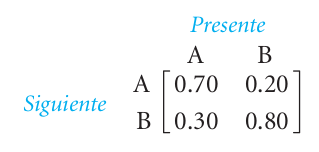
\includegraphics[width=0.9\textwidth]{imagenes/tabla}
					\[	
					\begin{array}{c@{}}
					\rowind{\color{blue}Siguiente} 
					\end{array}
					\begin{array}{c@{}c@{}}
					\rowind{\textbf{S}} \\ \rowind{\textbf{i}} 
					\end{array}
					\mathop{\left(
						\begin{array}{ *{2}{c} }
						\colind{0.7}{\textbf{S}}  &  \colind{0.2}{\textbf{i}} \\[0mm]			
						0.3 & 0.8    
						\end{array}
						\right)}^{
						\begin{array}{@{}c@{}}
						\rowind{\color{blue}Presente} \\ \mathstrut
						\end{array}
					}
					\]
				\end{figure}
			\end{column}
		\end{columns}	
		
		\vspace{5mm}
		\item Las columnas de $P$ son vectores de probabilidad (cualquier matriz cuadrada con esta propiedad se llama \textbf{\textit{matriz estocástica}}).
		
		\vspace{5mm}
		\item Si $P$ es matriz estocástica, entonces $P^2$ es estocástica (ejercicio).
		
		\vspace{5mm}
		\item ¿Es $P^2$ una matriz de transición del mismo tipo? ¿Qué representan sus entradas?
	\end{itemize}
	
\end{frame}
}

%%------------------------------------------------------------------------------------------------------

\subsection{}

{\nologo
\begin{frame}\frametitle{Observaciones sobre cadenas de Markov}
	
	\begin{itemize}\justifying 
		\item Sea $\left(P^k\right)_{ij}$ la entrada $ij$ de $P^k$. ¿Qué representa $\left(P^k\right)_{ij}$?
		
		\vspace{5mm}
		\item ¿Qué representa {\color{red}$\left(P^2\right)_{21}$}?
		
		\[
		P^2 =
		\left(
		\begin{array}{@{\hspace{0.2\tabcolsep}}c@{\hspace{1.2\tabcolsep}}c@{\hspace{0.2\tabcolsep}}}
		0.70 & 0.20 \\[1mm]
		0.30 & 0.80
		\end{array}
		\right)
		\left(
		\begin{array}{@{\hspace{0.2\tabcolsep}}c@{\hspace{1.2\tabcolsep}}c@{\hspace{0.2\tabcolsep}}}
		0.70 & 0.20 \\[1mm]
		0.30 & 0.80
		\end{array}
		\right)
		=
		\left(
		\begin{array}{@{\hspace{0.2\tabcolsep}}c@{\hspace{1.2\tabcolsep}}c@{\hspace{0.2\tabcolsep}}}
		0.55 & 0.30 \\[1mm]
		{\color{red}0.45} & 0.70
		\end{array}
		\right)
		\]		
	\end{itemize}
	
	\vspace{1mm}
	\begin{columns}[c]
		\begin{column}{0.2\textwidth}			
			\begin{figure}
				\centering
				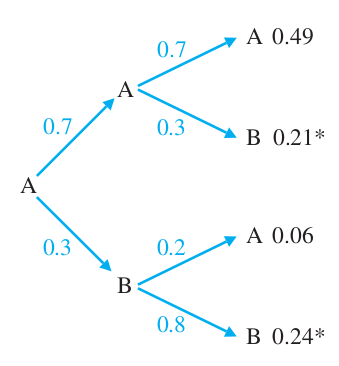
\includegraphics[width=1.5\textwidth]{imagenes/arbol}
			\end{figure}
			\vspace{1mm}
			
		\end{column}
		\hspace{3mm}
		\begin{column}{0.78\textwidth}
			\begin{itemize}
				\item Del estado $A$ se puede llegar al estado $B$ dos meses después de dos maneras
				distintas (marcadas con *)
				
				\vspace{3mm}
				\item La persona puede seguir usando $A$ después de 1 mes y luego cambiar a $B$ con probabilidad $0.7(0.3)= 0.21$
				
				\vspace{3mm}
				\item La persona puede cambiar a $B$ después de 1 mes y luego seguir con $B$ con probabilidad $0.3(0.8) = 0.24$.
				
				\vspace{3mm}
				\item La suma de estas probabilidades produce una probabilidad total de {\color{red}$0.45$}.
			\end{itemize}
		\end{column}
	\end{columns}
	
\end{frame}
}

%%------------------------------------------------------------------------------------------------------

\subsection{}

{\nologo
\begin{frame}\frametitle{Observaciones sobre cadenas de Markov}
	
	\begin{columns}[c]
		\begin{column}{0.2\textwidth}			
			\begin{figure}
				\centering
				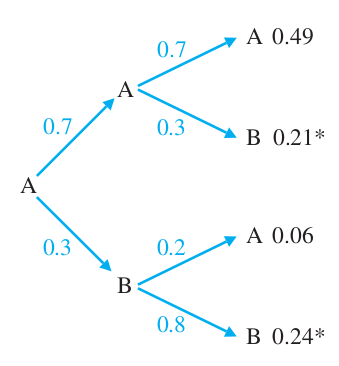
\includegraphics[width=1.5\textwidth]{imagenes/arbol}
			\end{figure}
			\vspace{1mm}
			
		\end{column}
		\hspace{3mm}
		\begin{column}{0.78\textwidth}
			\begin{itemize}
				\item Del estado $A$ se puede llegar al estado $B$ dos meses después de dos maneras
				distintas (marcadas con *)
				
				\vspace{3mm}
				\item La persona puede seguir usando $A$ después de 1 mes y luego cambiar a $B$ con probabilidad $0.7(0.3)= 0.21$
				
				\vspace{3mm}
				\item La persona puede cambiar a $B$ después de 1 mes y luego seguir con $B$ con probabilidad $0.3(0.8) = 0.24$.
				
				\vspace{3mm}
				\item La suma de estas probabilidades produce una probabilidad global de {\color{red}$0.45$}.
			\end{itemize}
		\end{column}
	\end{columns}
	
	\vspace{5mm}
	\begin{prop}{\textbf{Propiedad 1 }}\justifying
		$\left(P^k\right)_{ij}$ es la probabilidad de cambiar del estado $j$ al estado $i$ en $k$ transiciones.
	\end{prop}	
	
\end{frame}
}

%%------------------------------------------------------------------------------------------------------

\subsection{}

{\nologo
\begin{frame}%\frametitle{Observaciones (ejemplo 1)}
	
	\begin{ej}{\textbf{Ejemplo 1}}
		Hallar el número de usuarios de Samsung y iPhone en el mes $k$:
		\[
		\mathbf{x}_k = P^k\, \mathbf{x}_0 =
		\left(
		\begin{array}{@{\hspace{0.2\tabcolsep}}c@{\hspace{1.2\tabcolsep}}c@{\hspace{0.2\tabcolsep}}}
		0.70 & 0.20 \\[1mm]
		0.30 & 0.80
		\end{array}
		\right)^k
		\left(
		\begin{array}{@{\hspace{0.2\tabcolsep}}c@{\hspace{0.2\tabcolsep}}}
		120 \\[1mm]
		80
		\end{array}
		\right)
		= \ ?	
		\]
	\end{ej}	
	
	\textit{Solución.}
	
	\vspace{2mm}
	\begin{itemize}
		\item El polinomio característico de la \textit{matriz de transcición} A:
		
		\vspace{2mm}
		\[	
			p(\lambda) = |P-\lambda I| 
			=
			\left|	
			\begin{array}{@{\hspace{0.2\tabcolsep}}c@{\hspace{1.2\tabcolsep}}c@{\hspace{0.2\tabcolsep}}}
			0.7-\lambda & 0.2 \\[1mm]
			0.3 & 0.8-\lambda
			\end{array}
			\right| 
			=
			\lambda^2 - 1.5\lambda + 0.5		
		\]
		
		\vspace{6mm}
		\item Los valores propios de la \textit{matriz de transcición} A:
		
		\vspace{-0mm}
		\[
			\lambda^2 - 1.5\lambda + 0.5 =
			\left( \lambda - 0.5 \right) \left( \lambda - 1 \right) \ = \ 0 
			\quad  \Longrightarrow \quad   
			\lambda_1 = 0.5 \quad \text{y} \quad   \lambda_2 = 1
		\]				
		
	\end{itemize}
	
\end{frame}
}

%%------------------------------------------------------------------------------------------------------

\subsection{}


	\begin{frame}\frametitle{Espacios propios}
		
		\begin{itemize}
			\item Espacio propio $E_{\lambda_1}=E_{0.5}=N_{P-0.5I}$:
			
			\[				
			(A-0.5I \ | \ \mathbf{0})
			=
			\left(
			\begin{array}{@{\hspace{0.2\tabcolsep}}r@{\hspace{\tabcolsep}}r@{\hspace{\tabcolsep}}|r@{\hspace{0.2\tabcolsep}}}
			0.2 & 0.2 & 0  \\[1mm]
			0.3 & 0.3 & 0
			\end{array}
			\right) 
			\xrightarrow[]{\phantom{xx} }		
			\left(
			\begin{array}{@{\hspace{0.2\tabcolsep}}r@{\hspace{\tabcolsep}}r@{\hspace{\tabcolsep}}|r@{\hspace{0.2\tabcolsep}}}
			1 & 1 & 0  \\[1mm]
			0 & 0 & 0
			\end{array}
			\right) 
			\quad \Rightarrow \quad 
			\mathbf{v}_1 = 
			\left(
			\begin{array}{@{\hspace{0.3\tabcolsep}}r@{\hspace{0.5\tabcolsep}}}
			-1   \\[1mm]
			 1 
			\end{array}
			\right) 
			\]
			
			\vspace{6mm}
			\item  Espacio propio $E_{\lambda_2}=E_{1}=N_{P-I}$:
			
			\[				
			(A-I \ | \ \mathbf{0})
			=
			\left(
			\begin{array}{@{\hspace{0.2\tabcolsep}}r@{\hspace{1.2\tabcolsep}}r@{\hspace{\tabcolsep}}|r@{\hspace{0.2\tabcolsep}}}
			-0.3 & 0.2 & 0  \\[1mm]
			 0.3 & -0.2 & 0
			\end{array}
			\right) 
			\xrightarrow[]{\phantom{xx} }		
			\left(
			\begin{array}{@{\hspace{0.2\tabcolsep}}r@{\hspace{1.2\tabcolsep}}r@{\hspace{\tabcolsep}}|r@{\hspace{0.2\tabcolsep}}}
			3 & -2 & 0  \\[1mm]
			0 &    0 & 0
			\end{array}
			\right) 
			\quad \Rightarrow \quad 
			\mathbf{v}_2 = 
			\left(
			\begin{array}{@{\hspace{0.3\tabcolsep}}r@{\hspace{0.5\tabcolsep}}}
			2  \\[1mm]
			3 
			\end{array}
			\right) 
			\]
			
			\vspace{4mm}
			\item Condiciones iniciales del problema:
			
			\[	
			c_1\mathbf{v}_1 + c_2\mathbf{v}_2 = \mathbf{x}_0
			\quad \Rightarrow \quad 
			\left(
			\begin{array}{@{\hspace{0.2\tabcolsep}}r@{\hspace{1.4\tabcolsep}}r@{\hspace{\tabcolsep}}|c@{\hspace{0.2\tabcolsep}}}
			-1 & 2 & {\color{ForestGreen}120}  \\[2mm]
			 1 &  3 & {\color{ForestGreen}80}
			\end{array}
			\right) 
			\xrightarrow[]{\phantom{xx} }		
			\left(
			\begin{array}{@{\hspace{0.2\tabcolsep}}r@{\hspace{1.4\tabcolsep}}r@{\hspace{\tabcolsep}}|r@{\hspace{0.2\tabcolsep}}}
			1 & 0 & -40  \\[2mm]
			0 & 1 & 40
			\end{array}
			\right)  
			\]
			
		\end{itemize}
		
	\end{frame}


%%------------------------------------------------------------------------------------------------------

\subsection{}

{\nologo
\begin{frame}\frametitle{Información obtenida}
	
	%	$j_k$: número de hembras juveniles en el año $k$ (desde el inicio del estudio).
	%	$a_k$: número de hembras adultas en el año $k$ (desde el inicio del estudio).
	
	%	\vspace{2mm}
	\begin{itemize}
		
		\vspace{2mm}		
		\item Valores propios:
		
		\[	
		\lambda_1 = 0.5 \qquad \text{y} \qquad \lambda_2 = 1
		\]
		
		\vspace{8mm}
		\item Vectores propios:
		
		\vspace{1mm}
		\[	
		\mathbf{v}_1
		\ = \	
		\left(
		\begin{array}{@{\hspace{0.3\tabcolsep}}r@{\hspace{0.5\tabcolsep}}}
		-1   \\[1mm]
		 1 
		\end{array}
		\right) 
		\qquad \text{y} \qquad
		\mathbf{v}_2
		\ = \	
		\left(
		\begin{array}{@{\hspace{0.3\tabcolsep}}c@{\hspace{0.5\tabcolsep}}}
		2   \\[1mm]
		3 
		\end{array}
		\right) 
		\]
		
		\vspace{8mm}
		\item $A^{\color{red}k}\mathbf{x}_0 = c_1{\lambda_1}^{\color{red}k}\mathbf{v}_1 + c_2{\lambda_2}^{\color{red}k}\mathbf{v}_2$:
		
		\vspace{1mm}
		\[	
		\mathbf{x}_{\color{red}k}		
		\ = \				
		A^{\color{red}k}\mathbf{x}_0
		\ = \
		-40(0.5)^{\color{red}k}
		\left(
		\begin{array}{@{\hspace{0.3\tabcolsep}}r@{\hspace{0.5\tabcolsep}}}
		-1   \\[1mm]
		 1 
		\end{array}
		\right) 
		+
		40 
		\left(
		\begin{array}{@{\hspace{0.3\tabcolsep}}c@{\hspace{0.5\tabcolsep}}}
		2  \\[1mm]
		3 
		\end{array}
		\right) 
		\ = \
		-\frac{40}{2^{\color{red}k}}
		\left(
		\begin{array}{@{\hspace{0.3\tabcolsep}}r@{\hspace{0.5\tabcolsep}}}
		-1   \\[1mm]
		1 
		\end{array}
		\right) 
		+		
		\left(
		\begin{array}{@{\hspace{0.3\tabcolsep}}c@{\hspace{0.5\tabcolsep}}}
		80  \\[1mm]
		120 
		\end{array}
		\right) 
		\]
		
	\end{itemize}
	
\end{frame}
}

%%------------------------------------------------------------------------------------------------------

\subsection{}

{\nologo
\begin{frame}\frametitle{Vector estacionario}
	
	\vspace{-3mm}
	\begin{alertblock}{\textbf{Observación 1}}
		\begin{enumerate}[$a$]
			\item Los vectores de estado $\mathbf{x}_k$ se ``aproximan'' al vector $\mathbf{x}=(80, 120)$:
			\[
			\mathbf{x}_{k}
			\ = \
			-\frac{40}{2^{k}}
			\left(
			\begin{array}{@{\hspace{0.3\tabcolsep}}r@{\hspace{0.5\tabcolsep}}}
			-1   \\[1mm]
			1 
			\end{array}
			\right) 
			+		
			\left(
			\begin{array}{@{\hspace{0.3\tabcolsep}}c@{\hspace{0.5\tabcolsep}}}
			80  \\[1mm]
			120 
			\end{array}
			\right) 
			\to 
			\left(
			\begin{array}{@{\hspace{0.2\tabcolsep}}c@{\hspace{0.2\tabcolsep}}}
			80 \\[1mm]
			120
			\end{array}
			\right)
			\quad \text{cuando} \quad k\to \infty
			\]
			
			\vspace{0mm}
			\item $P\,\mathbf{x} = 
			\left(
			\begin{array}{@{\hspace{0.2\tabcolsep}}c@{\hspace{1.2\tabcolsep}}c@{\hspace{0.2\tabcolsep}}}
			0.70 & 0.20 \\[1mm]
			0.30 & 0.80
			\end{array}
			\right)
			\left(
			\begin{array}{@{\hspace{0.2\tabcolsep}}c@{\hspace{0.2\tabcolsep}}}
			80 \\[1mm]
			120
			\end{array}
			\right)
			=
			\left(
			\begin{array}{@{\hspace{0.2\tabcolsep}}c@{\hspace{0.2\tabcolsep}}}
			80 \\[1mm]
			120
			\end{array}
			\right)
			= \mathbf{x}$
		\end{enumerate}	
	\end{alertblock}	
	
	\vspace{-1mm}
	\begin{defi}{\textbf{Definición (vector de estado estacionario)}}\justifying
		Un vector de  estado $\mathbf{x}$ tal que $P \mathbf{x} = \mathbf{x}$ se llama 
		\textbf{\textit{vector de estado estacionario}}.
	\end{defi}
	
	\vspace{-1mm}
	\begin{alertblock}{\textbf{Observación 2}}
		\begin{enumerate}[$a$]\justifying 
			% \item Toda cadena de Markov tiene un vector de estado estacionario y es único (teorema).
			\item Toda cadena de Markov con matriz estocástica \textit{positiva} (todas sus entradas son positivas), 
			tiene un único vector de probabilidad estacionario.
			\item ¿Cómo hallar el vector de probabilidad de estado estacionario?
		\end{enumerate}
	\end{alertblock}	
	
\end{frame}
}

%%------------------------------------------------------------------------------------------------------

\subsection{}

{\nologo 
\begin{frame}\frametitle{Vector estacionario}
	
	\begin{ej}{\textbf{Ejemplo 2}}
		Halle el vector de probabilidad que es vector estacionario para esta cadena de Markov.
	\end{ej}	
	
	\textit{Solución.}
	
    
    \vspace{2mm}
	\begin{itemize}
		
		\item $\mathbf{x} \ \ \text{vector  estacionario} \ \ \Longleftrightarrow  \ \ P\mathbf{x}=\mathbf{x} 
		\ \  \Longleftrightarrow \ \ (P-I)\mathbf{x}=\mathbf{0}$.
		
		\vspace{8mm}
		\item $
		(P-I \ | \ \mathbf{0})
		=
		\left(
		\begin{array}{@{\hspace{0.2\tabcolsep}}r@{\hspace{\tabcolsep}}r@{\hspace{\tabcolsep}}|r@{\hspace{0.2\tabcolsep}}}
			-0.3 &  0.2 & 0  \\[1mm]
			 0.3 & -0.2 & 0
		\end{array}
		\right) 
		\xrightarrow[]{\phantom{xx} }		
		\left(
		\begin{array}{@{\hspace{0.2\tabcolsep}}r@{\hspace{\tabcolsep}}r@{\hspace{\tabcolsep}}|r@{\hspace{0.2\tabcolsep}}}
			3 & -2 & 0  \\[1mm]
			0 & 0 & 0
		\end{array}
		\right) 
		\quad \Rightarrow \quad 
		\mathbf{x} = 
		\left(
		\begin{array}{@{\hspace{0.3\tabcolsep}}c@{\hspace{0.3\tabcolsep}}}
			\frac{2}{3}t   \\[1mm]
			t 
		\end{array}
		\right) 
		$
		
		\vspace{8mm}
		\item $\mathbf{x} \ \ \text{es vector de probabilidad} \ \ \Leftrightarrow  \ \ \frac{2}{3}t+t=1
		\ \  \Leftrightarrow \ \ \mathbf{x} = 
		\left(
		\begin{array}{@{\hspace{0.3\tabcolsep}}r@{\hspace{0.5\tabcolsep}}}
		\frac{2}{5}   \\[2mm]
		\frac{3}{5} 
		\end{array}
		\right) 
		=
		\left(
		\begin{array}{@{\hspace{0.3\tabcolsep}}r@{\hspace{0.5\tabcolsep}}}
		0.4   \\[2mm]
		0.6
		\end{array}
		\right) 
		$
		
	\end{itemize}
	
\end{frame}
}